\section{Data System Architecture – Explanation}

\begin{figure}[H]
  \centering
  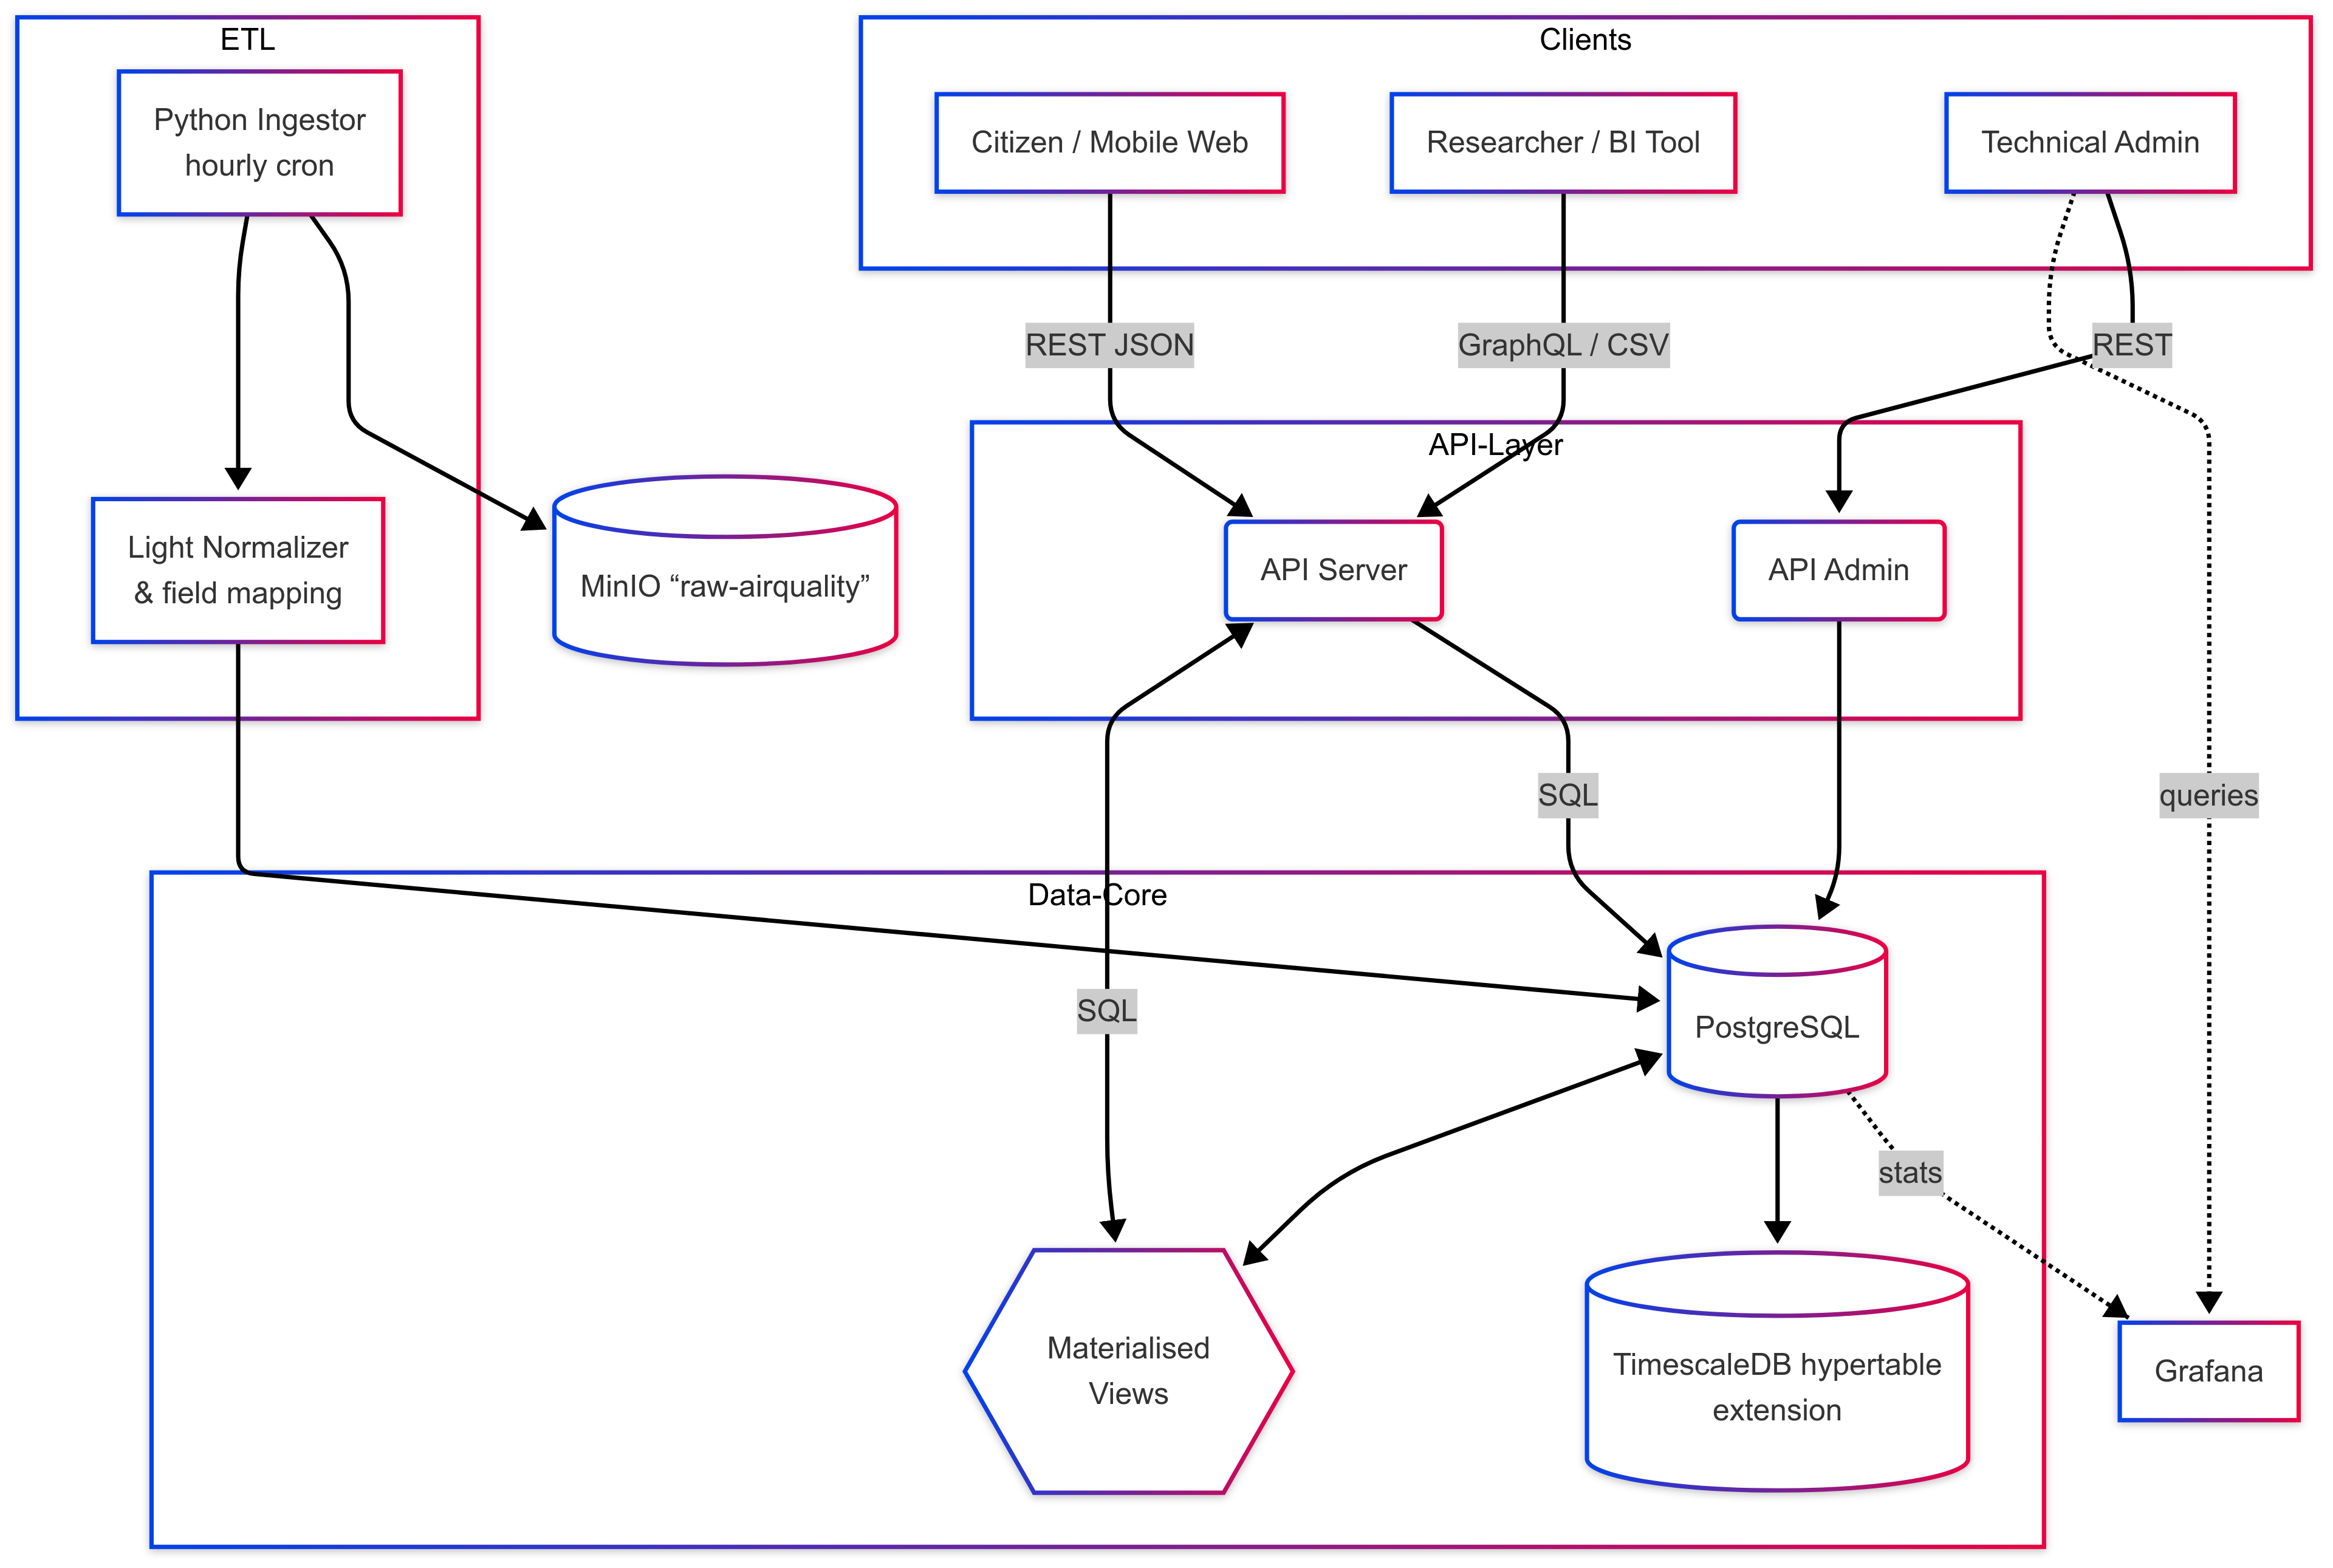
\includegraphics[width=0.8\textwidth]{Imagenes/Arquitectura.png}
  \caption{High-level architecture diagram}
\end{figure}

\subsection*{1. Ingestion and Raw Storage}
A lightweight Python service (\textbf{Ingestor}) polls air quality endpoints at regular intervals. Each JSON payload is first persisted—unchanged—in a MinIO bucket (\texttt{raw-airquality}) to ensure auditability and allow for future replay.

\subsection*{2. Normalization and Relational Store}
A mapping layer converts heterogeneous field names, units, and AQI scales into a unified schema before inserting the data into a partitioned PostgreSQL database. Monthly partitions, created using TimescaleDB, reduce index scan sizes and ensure sub-second query performance for time-localized filters.

\subsection*{3. Query Acceleration}
Materialized views are refreshed concurrently to avoid blocking read operations, providing fast access to aggregated insights.

\subsection*{4. API and User Access}
An API layer exposes REST and GraphQL endpoints for citizens, researchers, and BI tools. Administrative users access the database through a dedicated API, while query latency and slow statements are monitored via Grafana dashboards.
\newpage